
% Template for Elsevier CRC journal article
% version 1.0 dated 13 October 2009

% This file (c) 2009 Elsevier Ltd.  Modifications may be freely made,
% provided the edited file is saved under a different name

% This file contains modifications for Procedia Computer Science

%%%%%%%%%%%%%%%%%%%%%%%%%%%%%%%%%%%%%%%%%%%%%%%%%%%%%%%%%%%%%%%%%%%%%%%%%%

%% This template uses the elsarticle.cls document class and the extension package ecrc.sty
%% For full documentation on usage of elsarticle.cls, consult the documentation "elsdoc.pdf"
%% Further resources available at http://www.elsevier.com/latex

%%%%%%%%%%%%%%%%%%%%%%%%%%%%%%%%%%%%%%%%%%%%%%%%%%%%%%%%%%%%%%%%%%%%%%%%%%

%% The '1p' and 'times' class options of elsarticle are used for Elsevier CRC
\documentclass[1p,times]{elsarticle}

%% The `ecrc' package must be called to make the CRC functionality available
\usepackage{ecrc}

%% The ecrc package defines commands needed for running heads and logos.
%% For running heads, you can set the journal name, the volume, the starting page and the authors

%% set the volume if you know. Otherwise `00'
\volume{00}

%% set the starting page if not 1
\firstpage{1}

%% Give the name of the journal
\journalname{Procedia Computer Science}

%% Give the author list to appear in the running head
%% Example \runauth{C.V. Radhakrishnan et al.}
\runauth{M. Rivi et al.}

%% The choice of journal logo is determined by the \jid and \jnltitlelogo commands.
%% A user-supplied logo with the name <\jid>logo.pdf will be inserted if present.
%% e.g. if \jid{yspmi} the system will look for a file yspmilogo.pdf
%% Otherwise the content of \jnltitlelogo will be set between horizontal lines as a default logo

%% Give the abbreviation of the Journal.
\jid{procs}

%% Give a short journal name for the dummy logo (if needed)
\jnltitlelogo{Procedia Computer Science}

%% Hereafter the template follows `elsarticle'.
%% For more details see the existing template files elsarticle-template-harv.tex and elsarticle-template-num.tex.

%% Elsevier CRC generally uses a numbered reference style
%% For this, the conventions of elsarticle-template-num.tex should be followed (included below)
%% If using BibTeX, use the style file elsarticle-num.bst

%% End of ecrc-specific commands
%%%%%%%%%%%%%%%%%%%%%%%%%%%%%%%%%%%%%%%%%%%%%%%%%%%%%%%%%%%%%%%%%%%%%%%%%%

%% The amssymb package provides various useful mathematical symbols
\usepackage{amssymb}
%% The amsthm package provides extended theorem environments
%% \usepackage{amsthm}

%% The lineno packages adds line numbers. Start line numbering with
%% \begin{linenumbers}, end it with \end{linenumbers}. Or switch it on
%% for the whole article with \linenumbers after \end{frontmatter}.
%% \usepackage{lineno}

%% natbib.sty is loaded by default. However, natbib options can be
%% provided with \biboptions{...} command. Following options are
%% valid:

%%   round  -  round parentheses are used (default)
%%   square -  square brackets are used   [option]
%%   curly  -  curly braces are used      {option}
%%   angle  -  angle brackets are used    <option>
%%   semicolon  -  multiple citations separated by semi-colon
%%   colon  - same as semicolon, an earlier confusion
%%   comma  -  separated by comma
%%   numbers-  selects numerical citations
%%   super  -  numerical citations as superscripts
%%   sort   -  sorts multiple citations according to order in ref. list
%%   sort&compress   -  like sort, but also compresses numerical citations
%%   compress - compresses without sorting
%%
%% \biboptions{comma,round}

% \biboptions{}

% if you have landscape tables
%%%\usepackage[figuresright]{rotating}

% put your own definitions here:
%   \newcommand{\cZ}{\cal{Z}}
%   \newtheorem{def}{Definition}[section]
%   ...

% add words to TeX's hyphenation exception list
%\hyphenation{author another created financial paper re-commend-ed Post-Script}

% declarations for front matter

\newcommand{\aj}{AJ}
\newcommand{\apj}{ApJ}
\newcommand{\apjl}{ApJ}
\newcommand{\apjs}{ApJS}
\newcommand{\aap}{A\&A}
\newcommand{\aaps}{A\&AS}
\newcommand{\mnras}{MNRAS}
\newcommand{\nat}{Nature}
\newcommand{\araa}{ARAA}
\newcommand{\prd}{Phys. Rev. D}
\newcommand{\pasj}{PASJ}
\newcommand{\pasp}{PASP}
\newcommand{\physrep}{Phys. Rep.}


\begin{document}

\begin{frontmatter}

%% Title, authors and addresses

%% use the tnoteref command within \title for footnotes;
%% use the tnotetext command for the associated footnote;
%% use the fnref command within \author or \address for footnotes;
%% use the fntext command for the associated footnote;
%% use the corref command within \author for corresponding author footnotes;
%% use the cortext command for the associated footnote;
%% use the ead command for the email address,
%% and the form \ead[url] for the home page:
%%
%% \title{Title\tnoteref{label1}}
%% \tnotetext[label1]{}
%% \author{Name\corref{cor1}\fnref{label2}}
%% \ead{email address}
%% \ead[url]{home page}
%% \fntext[label2]{}
%% \cortext[cor1]{}
%% \address{Address\fnref{label3}}
%% \fntext[label3]{}

\dochead{}
%% Use \dochead if there is an article header, e.g. \dochead{Short communication}



\title{High Performance Visualization of astrophyisical data using Splotch}

%% use optional labels to link authors explicitly to addresses:
%% \author[label1,label2]{<author name>}
%% \address[label1]{<address>}
%% \address[label2]{<address>}

\author{Marzia Rivi}
\ead{m.rivi@cineca.it}
\address{CINECA, Via Magnanelli 6/3, Casalecchio di Reno, Italy}

\author{Zhefan Jin}
\ead{Zhefan.Jin@port.ac.uk}
\address{...}

\author{Klaus Dolag}
\ead{kdolag@MPA-Garching.MPG.DE}
\address{Max-Planck-Institut f\"ur Astrophysik, Karl-Schwarzschild Strasse 1, Garching bei M\"unchen, Germany}

\author{Claudio Gheller }
\ead{c.gheller@cineca.it}
\address{CINECA, Via Magnanelli 6/3, Casalecchio di Reno, Italy}

\author{Mel Krokos }
\ead{mel.krokos@port.ac.uk}
\address{...}

\begin{abstract}

.........

\end{abstract}

\begin{keyword}
%% keywords here, in the form: keyword \sep keyword


Visualization \sep High Performance Computing \sep Astrophysics

%% PACS codes here, in the form: \PACS code \sep code

%% MSC codes here, in the form: \MSC code \sep code
%% or \MSC[2008] code \sep code (2000 is the default)

\end{keyword}

\end{frontmatter}

%%
%% Start line numbering here if you want
%%
% \linenumbers

\section{Introduction}
\label{intro}

Data represents a critical issue for scientists and, in particular, astronomers. 
Observational instruments (telescopes, satellites...) produce enormous quantities of images and information. 
Computers and numerical simulations generate huge amount of data. All these data must be stored, 
managed and analyzed. These steps require great human effort, large scale facilities and efficient, powerful tools.  
Knowledge-discovery and data mining software often offer an efficient
instrument for automatically exploring large volumes of data. However, the most immediate,
intuitive and effective way to discover and understand the properties of data
is provided by {\it visualization}. Visualization leads the user to quickly
focus on the interesting characteristics of a system. It allows
 different properties of the data to be shown simultaneously, and it can allow the user 
to navigate inside the data. Visualization is the most natural way of finding correlations, 
similarities and patterns. It is an effective method for
selecting special regions or features, on which the researcher can concentrate his/her
efforts and the subsequent quantitative analysis. Finally, visualization is 
useful to get a quick look at an ongoing processes, e.g. a numerical simulation, 
in order, for instance, to monitor it and to understand if its behavior is as expected or if
something is going wrong and, in that case, to correct it saving time and resources.\\
For these reasons, the astronomical community has always dedicated special
attention to the growth of graphical and visualization tools, driving their evolution or even being
directly involved in the development of many of them.
At present, the most popular software for astronomers can be subdivided
into two main categories: tools for image display and processing and tools for
plotting data. Notable among the former are IRAF, by NOAO; ESO-MIDAS, by the 
European Southern Observatory; SaoImage, by the Smithsonian Astrophysical Observatory and
GAIA, by ESO. Many other tools are available, but we refer to dedicated surveys
for a complete list. Gnuplot and SuperMongo are 
popular applications adopted for 2D data plots. A more sophisticated solution 
is represented by IDL, by ITT Visual Information, which is characterized
by a large library of functions specifically developed for astrophysics. 

The last generation 
of tools, like ParaView (cite), VisIVO (cite), VisIT (cite), Aladin
(cite) have been developed to overcome the limits
and the barriers of traditional software by exploiting the latest technological 
opportunities. Again, for a complete list, we refer to specific surveys. 

In this paper we present the High Performance Computing implementation of
Splotch \citep{2008NJPh...10l5006D}, a ray-tracing software designed to visualize data coming from particle 
based computer simulations. Cosmological N-Body simulations represents a paradigmatic
example of such applications. They account for some of the largest simulations in astrophysics, 
as, for instance, the MillenniumII simulation (cite), which describe the evolution 
of a meaningful fraction of the universe by means of 10 billions of fluid elements
(particles) interacting via gravitational forces. Each output of the MillenniumII 
\citep{2009MNRAS.398.1150B} simulation is about 400 Gbyte of data representing the 
3D position and the velocity of the particles, their ID and some additional, calculated
properties like the local smoothing length (e.g. distance wich contains 32 neighbours),
local density or local velocity dispersion. The manipulation of this dataset is feasibile 
only if high performance computing (HPC) resources are adopted. 

The sequential version of Splotch \citep{2008NJPh...10l5006D} has been re-designed and extended in order
to exploit both multiprocessor and multi-GPUs architectures currently available. 
A Single Instruction Multiple Data (SIMD) approach has been adopted for the parallelization
of the Splotch core algorithms, adopting the MPI library to support distributed multicore systems, 
OpenMP for shared memory nodes and CUDA for exploiting NVIDIA GPU systems. The different 
solutions can be used jointly on hybrid architectures. The details and
the benchmarks of such high performance implementation will be presented in the following sections.  


\section{The Splotch Algorithm}
\label{splotch}

\begin{figure}
\begin{center}
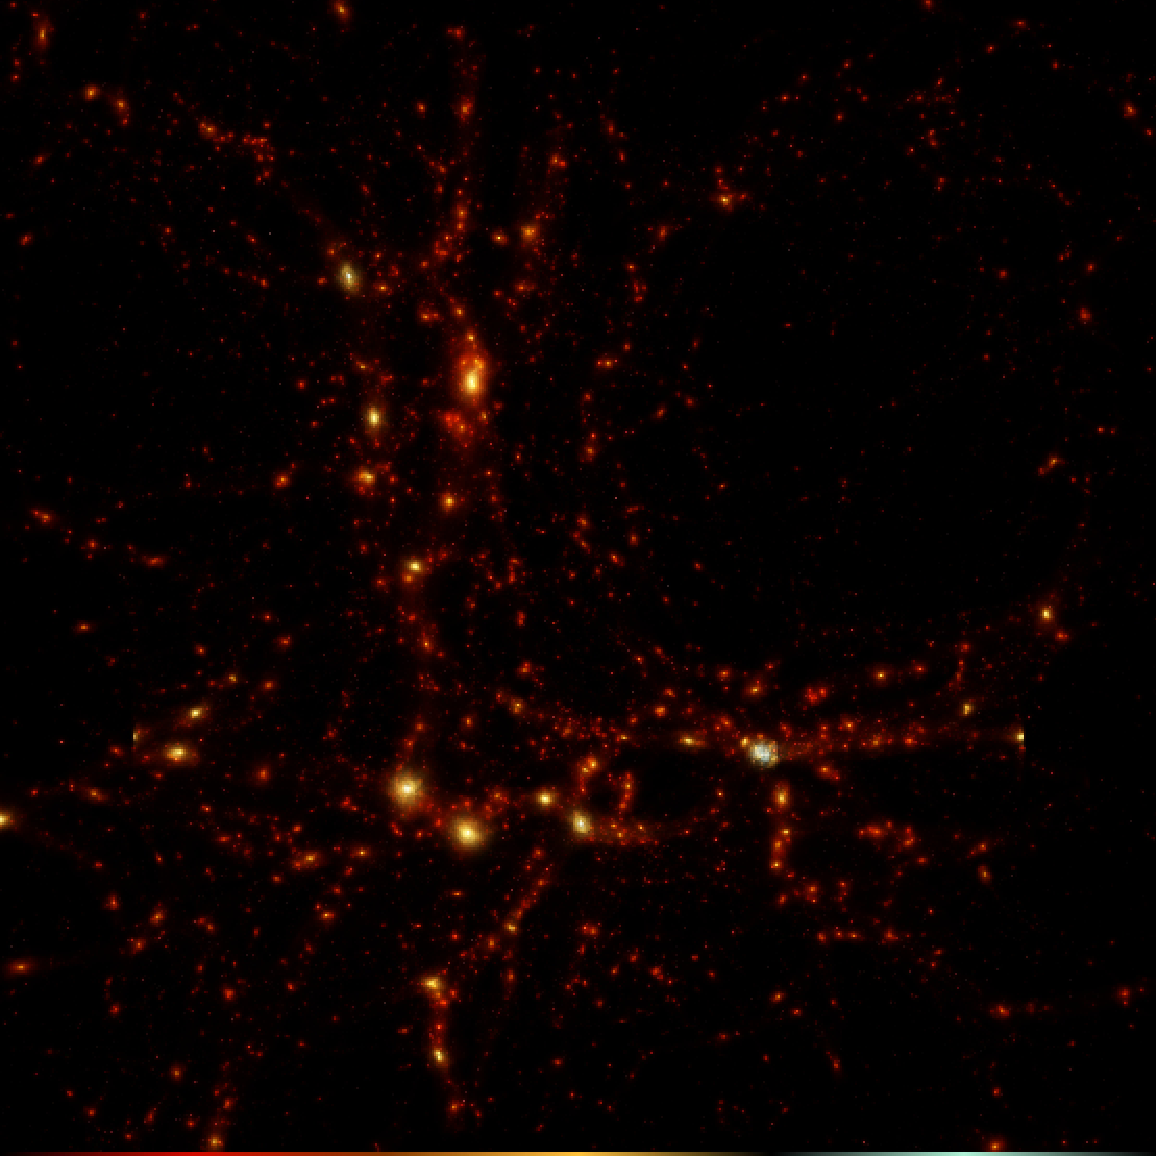
\includegraphics[width=0.49\textwidth]{millenium2_veldisp.pdf}
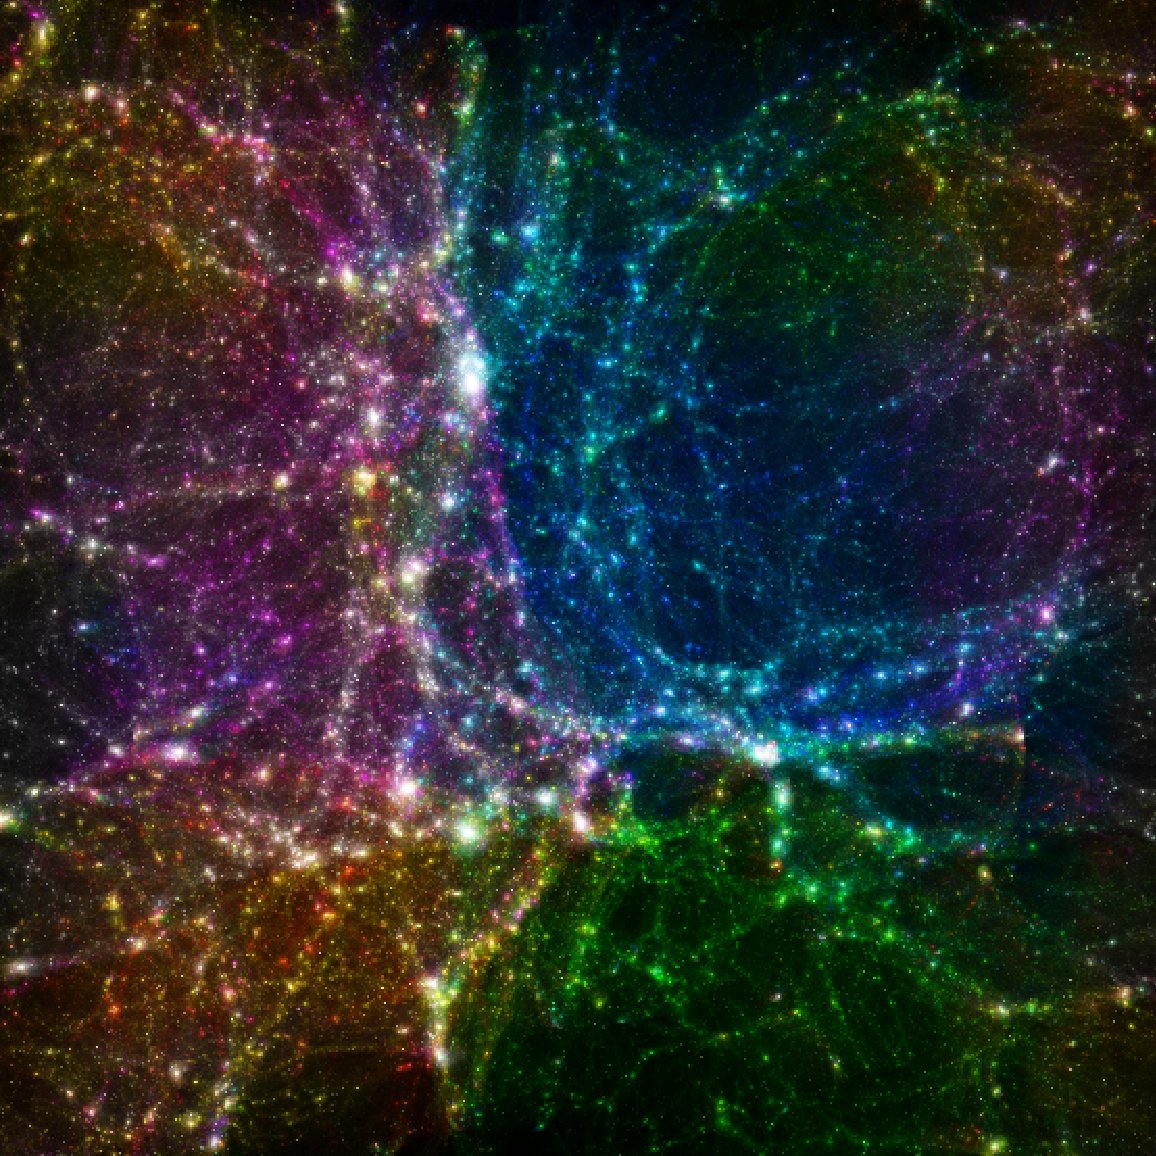
\includegraphics[width=0.49\textwidth]{millenium2_vel.pdf}
\end{center}
\caption{Shown are vizualisation of the MilleniumII simulation \citep{2009MNRAS.398.1150B} using
the velocity dispersion (left panel) and the three dimensional velocity (right panel) of the
particles for the color transfere function. The inlay shows a zoom on one the most rich structure
inside the simulation.}\label{mil2}
\end{figure}

The rendering algorithm of {\tt Splotch} is generally designed to handle
point-like particle distributions. Such tracer particles can be smoothed
to obtain a contineous field, most commonly the $B_2$-Spline \citep{1985A&A...149..135M}
\begin{equation}
   W(x,h)=\frac{8}{\pi h^3}\left\{\begin{array}{ll}
      1 - 6 \left(\frac{x}{h}\right)^2 + 6 \left(\frac{x}{h}\right)^3 \;\;& 0 \le \frac{x}{h} < 0.5 \\
      2 \left(1 - \frac{x}{h}\right)^3                              & 0.5 \le \frac{x}{h} < 1 \\
      0                                                             & 1 \le \frac{x}{h} \\
   \end{array} \right. , \label{SPH:kern}
\end{equation}
where $h$ is the local smoothing length, which is typically defined in a way
that every particle overlaps with $\approx 32$ neighbors. Therefore, the rendering is
based on the following assumptions:

\begin{itemize}
\item The contribution to the matter density by every particle can
be described as a Gaussian distribution of the form 
$\rho_p(\vec r)=\rho_{0,p}\exp(-r^2/\sigma_p^2)$.\footnote{Note that the
$b_2$-Spline kernel used in SPH has a shape very similar to the Gaussian distribution.} In
practice, it is much more handy to have a compact support of the
distribution, and therefore the distribution is set to zero at a given
distance of $f\cdot\sigma_p$. Following the approach often used to vizualice 
cosmological simulation we choose $f$ in such a way that
$f\cdot\sigma_p$ is related to the smoothing length $h$, i.e.
to fulfill $h \approx f\cdot\sigma_p$. Therefore rays passing
the particle at a distance larger than $f\cdot\sigma_p$ will be practically
unaffected by the particle's density distribution.
\item We use three ``frequencies'' to describe the red, green and blue
components of the radiation, respectively. These are treated independently.
\item The radiation intensity $\bf{I}$\footnote{Here we treat all
intensities as vectors with r,g and b components.} along a ray through the simulation
volume is modeled by the well known radiative transfer equation
\begin{equation}
\frac{d\bf{I}(x)}{dx}=(\bf{E}_p-\bf{A}_p\bf{I}(x))\rho_p(x),
\end{equation}
which can be found in standard textbooks like \citet{1991par..book.....S}.
Here, $\bf{E}_p$ and $\bf{A}_p$ describe the strength of radiation emission and absorption
for a given particle for the three rgb-colour components. In general it is recommended to
set $\bf{E}_p=\bf{A}_p$, which typically produces visually appealing images; for special
effects, however, independent emission and absorption coefficients can be used. Specially typically
a small gray component (e.g. a small, constant addition to the rgb-components) can be added 
to the absortpion of each particle ($\bf{A}_p$) to improve the three dimensional impression.
In general the coefficients can vary between particles, and are typically chosen as a function 
of a characteristic particle property. If a scalar quantity is choosen (e.g. the particle temperature, 
density, velocity dispersion, etc.), the mapping to the three components of $\bf{E}$ and $\bf{A}$ (for red, green and blue)
is typically achieved via a transfere function, realized by a colour look-up table or palette, which can
be provided to the ray-tracer as an external file to allow a maximum of flexibility. If a
vector quantity is chosen (r.g. velocity, magnetic field, etc.), the three components of the vectors
can be maped to the three components of $\bf{E}$ and $\bf{A}$ (for red, green and blue). Additional 
to the color, the intensity of each particle can be aditional modulated proportional to another
scalar property (e.g. density, etc.).
\end{itemize}

Assuming that absorption and emission are homogeneously mixed it
can be shown that, whenever a ray traverses a particle, its intensity
change is given by
\begin{equation}
\label{i_change}
\bf{I}_{\mbox{after}}=(\bf{I}_{\mbox{before}}-\bf{E}_p/\bf{A}_p)\exp(-\bf{A}_p\int_{-\infty}^\infty\rho_p(x)dx) + \bf{E}_p/\bf{A}_p
\end{equation}
The integral in this equation is given by
$\rho_{0,p}\sigma_p\exp{(-d_0^2/\sigma_p^2)}\sqrt{\pi}$, where $d_0$
is the minimum distance between the ray and the particle center.

Under the assumption that the particles do not overlap, the intensity
reaching the observer could simply be calculated by applying this formula to
all particles intersecting with the ray, in the order of decreasing distance
to the observer. In reality, of course, the particles do overlap, but since
the relative intensity changes due to a single particle can be assumed to be
very small, this approach can nevertheless be used in good approximation.

Figure \ref{mil2} shows a vizualisation example of a large simulation 
containing 10 billion particles.

\section{Parallel Implementation}
\label{parallel}

The Splotch code workflow consists in a number of steps which can be summarized as follows:

\noindent 1. Read data from one or more files;

\noindent 2. process data for rescaling, normalization etc.;

\noindent 3. render data;

\noindent 4. save the final image.

All these steps can be parallelized according to the same strategy, based on a SIMD approach. 
This consists in 
distributing the data in a balanced way between the different computing elements.
Each computing element performs the same operations on its subset of data contributing 
to the final (unique) image. 

The parallel implementation has been accomplished using different approaches, suitable 
for different hardware architectures and software environments. The MPI library (cite) 
has been used to define the overall data and work distribution characterization. Data are
read in chuncks of the same (or similar) size from each processor in the MPI pool. Then 
the same work is performed for steps 2 and 3 on the chuncks by each processor. Finally,
the final image is generated and saved only in the master processor, since this is a 
light task, which does not require any kind of parallel implementation. The work accomplished
in steps 2 and 3 can be further split, exploiting multicore shared memory processors or Graphic Cards.
In the first case, an OpenMP (cite) based approach provides the necessary parallelization tools. 
In the second case, the CUDA programming language has been adopted. The different approaches
can be used separately, if the available computing system fits only one of the available 
configurations, or jointly. For instance, on a single core PC with an NVIDIA graphic card, 
only the CUDA based parallelization strategy can be activated and exploited. On a multicore
RVN (cite) node both MPI and CUDA can be used. This makes the parallel Splotch code extremely 
flexible, portable, efficient and scalable.


\subsection{MPI Implementation}
\label{mpi}

Once the data is properly distributed among the processors, all the remaining operations 
are performed locally and further communiction is not needed, until the generation
of the final result. Each MPI process uses the assigned 
data to produce its own partial image. At the end, all the partial contributes are merged by means of a 
collective reduction operation producing the final image. 

The data load stage represents the crucial step for balancing the workload and for fast reading 
data from the disk. In fact, from the results presented in section x.x, it is clear how,
as the data size grows,
the data load process tends to be the most demanding section of the code. For this reason,
we have paied specific attention to the effective implementations of this functionality.

The adoption of MPI I/O (cite) based functions, represents the ideal solution for obtaining 
a high-performance and scalable read utility. However, an alternative solution is required, in
order to support high performance computing environments where MPI I/O is not available. 



\subsection{CUDA Implementation}
\label{cuda}

\section{Benchmarks}
\label{bench}

\begin{figure}
\begin{center}
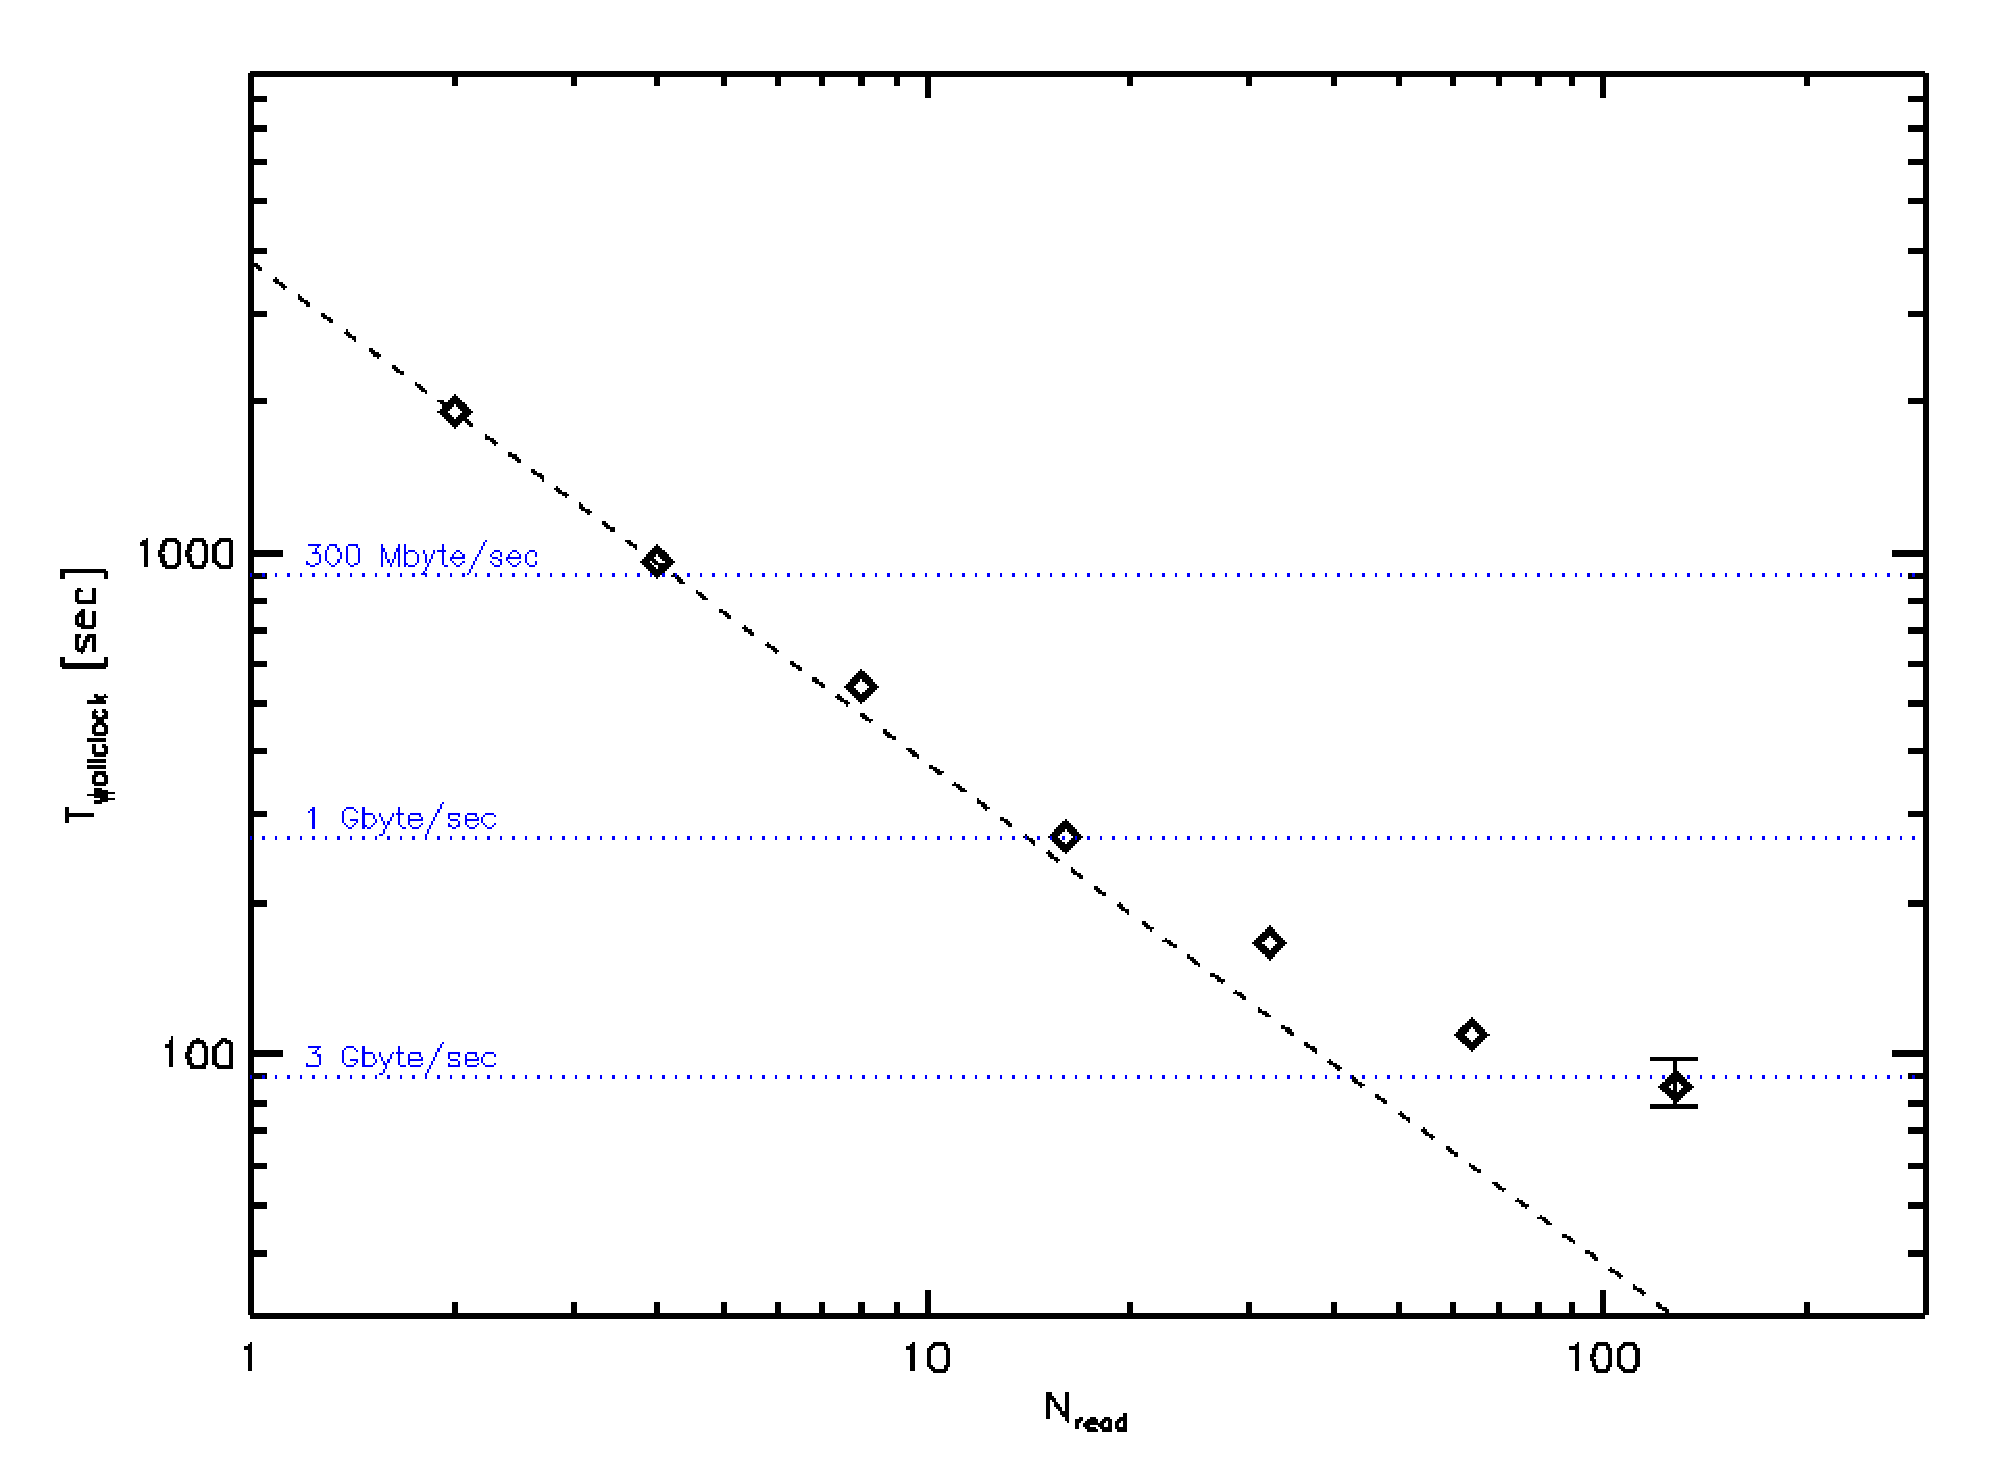
\includegraphics[width=0.5\textwidth]{t_cpu.pdf}
\end{center}
\caption{Shown is the scaling of the CPU time (total wallclock time substracting the time needed for 
readind and writing) with the number of MPI threads used for vizualisng 10 billion particles with an final
image size of 3200x3200 pixels. The dashed line indicates the expectation for an ideal scaling. The test was 
performed on a {\it Power6} architecture. The diamonds are runs using one task per core, the triangles indicate
using two tasks per core (a special feature of the {\it Power 6} architecture), where we measure a speedup of 
a factor of 1.4.}\label{cpu_scaling}
\end{figure}

\begin{figure}
\begin{center}
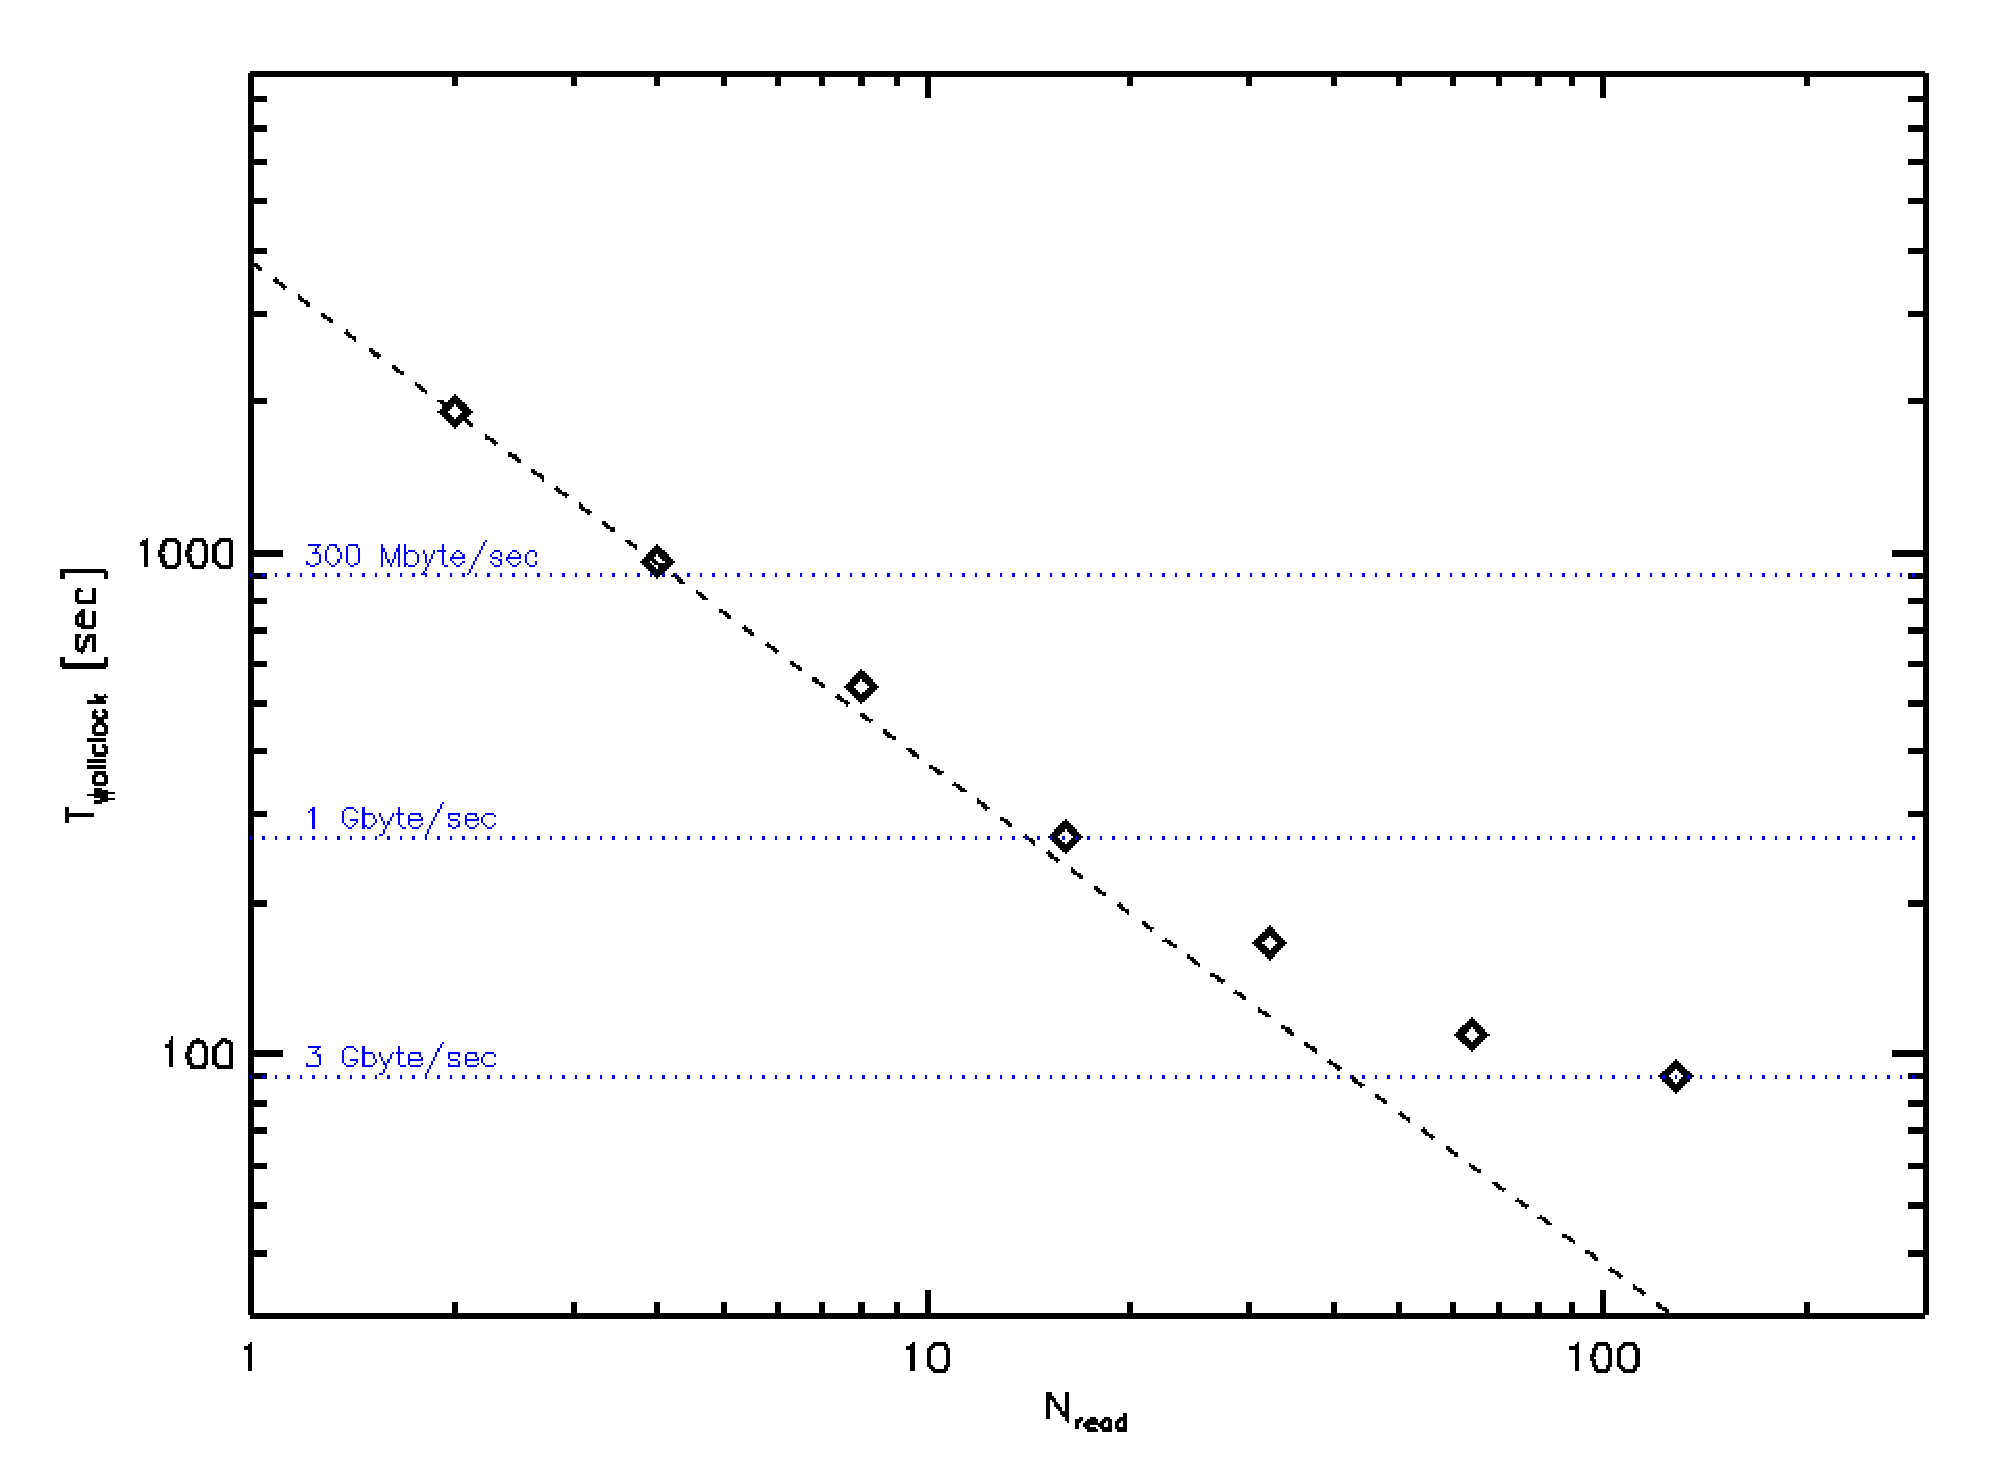
\includegraphics[width=0.5\textwidth]{t_read.pdf}
\end{center}
\caption{Shown is the scaling of the allclock time needed to read the needed data 
(position, velocity and smoothing length) for the 10 billion particles of the simulation
as function of parallel reading tasks. The dashed line indicates the expectation for an 
ideal scaling. The horizontal lines indicate time expected for and IO throughput of 300 Mbype/sec,
1 Gbyte/sec and 3 Gbyte/sec. The read datapoint indicate the reading speed obtained if naively 
individual data elements are streamed instead of reading large blocks in juncks.}\label{read_scaling}
\end{figure}


\section{Conclusions}
\label{conclusions}

\section*{Acknowledgments}
We would like to thank Mike for providing the data of the MilleniumII simulations 
on which we conducted our perfgomance tests. K.~D.~acknowledges the
supported by the DFG Priority Programme 117.

\section*{References}

%% The Appendices part is started with the command \appendix;
%% appendix sections are then done as normal sections
%% \appendix

%% \section{}
%% \label{}

%% References
%%
%% Following citation commands can be used in the body text:
%% Usage of \cite is as follows:
%%   \cite{key}         ==>>  [#]
%%   \cite[chap. 2]{key} ==>> [#, chap. 2]
%%

%% References with BibTeX database:

\bibliographystyle{elsarticle-num}
\bibliography{master.bib}

%% Authors are advised to use a BibTeX database file for their reference list.
%% The provided style file elsarticle-num.bst formats references in the required Procedia style

%% For references without a BibTeX database:

% \begin{thebibliography}{00}

%% \bibitem must have the following form:
%%   \bibitem{key}...
%%

% \bibitem{}

% \end{thebibliography}

\end{document}

%%
%% End of file `procs-template.tex'. 
